\documentclass[10pt]{article}
\usepackage[a4paper,margin=18mm]{geometry}
\usepackage{graphicx}
\usepackage{float}
\usepackage{booktabs}
\usepackage{array}
\usepackage{hyperref}
\usepackage{xcolor}
\usepackage{amsmath}
\usepackage{url}

\hypersetup{colorlinks=true,linkcolor=blue!50!black,urlcolor=blue!50!black}
\urlstyle{same}
\graphicspath{{figures/}}
\setlength{\parindent}{0pt}
\setlength{\parskip}{5pt}

\title{CD-A Niche 4 Domain-KL 100-Mode Inversion\\Three-Hour Native OGS Campaign}
\author{Generated from \texttt{inversion\_atempt}}
\date{2026-06-08}

\begin{document}
\maketitle

\section*{Executive Summary}

This report records the completed 365-day native OGS campaign
\texttt{ert10\_support\_365d\_domain\_kl\_100\_3h\_native\_s1\_v1}. The
campaign ran 16 parallel Metropolis-Hastings chains with a 100-mode 2D
domain-KL intrinsic-permeability magnitude field. The run completed cleanly,
wrote \texttt{campaign\_samples.csv} and \texttt{campaign\_manifest.json}, and
left no live OGS worker processes for this campaign.

The best ERT candidate is \texttt{chain06\_step0039\_proposal}. Its fitted
open-niche hydraulic-boundary time shift is \textbf{+89.035 days}. The 10-point
ERT objective is 0.278451 and the 10-point mean absolute residual is 0.071674
in log10 resistivity. On the independent 100-point circular ERT diagnostic, the
mean annual MAE is 0.101334 log10, compared with 0.111878 for the previous
rough-RF baseline, improving 62 of 100 circular supports.

\section{Campaign Status}

\begin{table}[H]
\centering
\begin{tabular}{ll}
\toprule
Quantity & Value \\
\midrule
Campaign rows & 1221 \\
Manifest wall time & 10912.413 s \\
Requested max wall time & 10800.0 s \\
Horizon & 365 days \\
Backend & native \\
Parallel chains & 16 \\
Best ERT candidate & \texttt{chain06\_step0039\_proposal} \\
\bottomrule
\end{tabular}
\caption{Completed campaign status. The small wall-time overrun is expected because the runner waits for in-flight OGS calls before writing final files.}
\end{table}

\section{Setup And Smoke Gates}

Before the 3-hour campaign, the new 100-mode domain-KL field was fitted to the
previous rough-RF best field and smoke-tested through native OGS. The KL
coefficient gate was \(|\xi|<6\); the fitted approximation passed with maximum
\(|\xi|=3.78037\) and p95 \(|\xi|=1.53246\). The native smoke run had ERT
objective 0.364329 and ERT MAE 0.090837.

\begin{figure}[H]
\centering
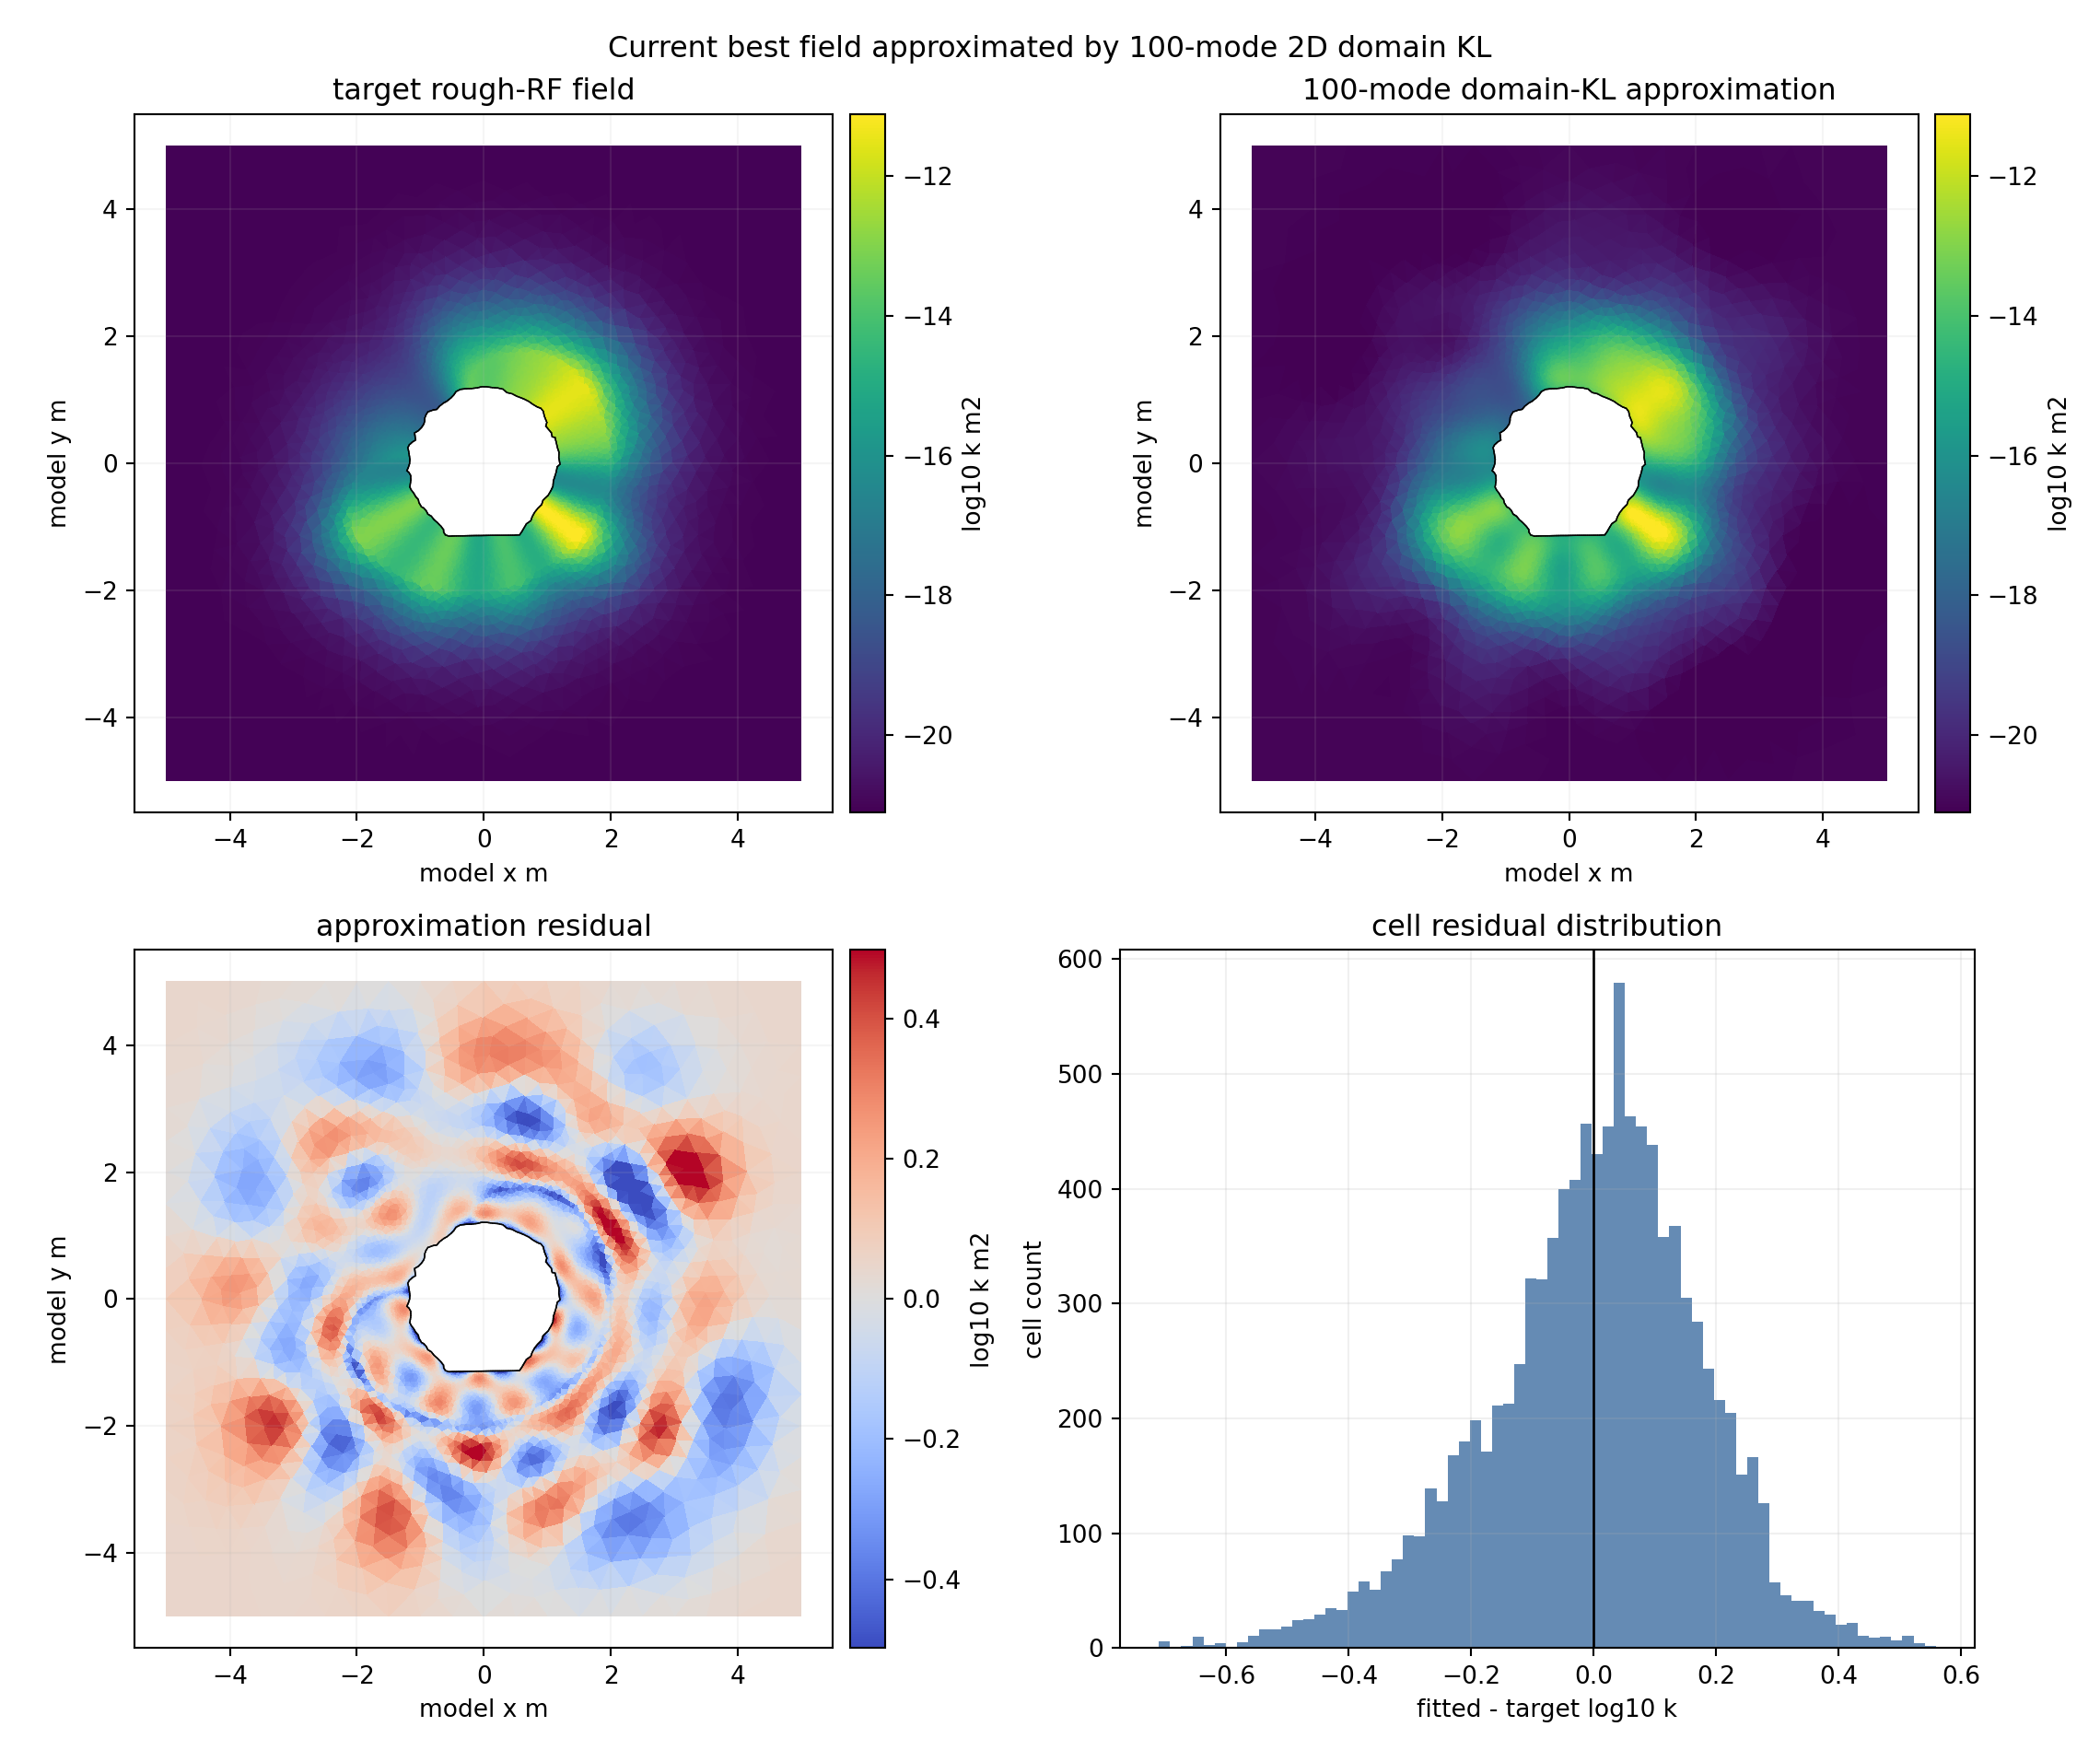
\includegraphics[width=0.94\linewidth]{domain_kl_fit_to_current_best_field.png}
\caption{Domain-KL approximation of the previous rough-RF best permeability field before the full campaign.}
\end{figure}

\section{Parameterization And Priors}

The active OGS field is tensor-valued intrinsic permeability
\texttt{k\_i\_rd}. The domain-KL random field controls only the scalar log10
magnitude. The tensor written to OGS is
\[
K_i(x)=R(\alpha)\left(10^{k_0 + \sigma_f\sum_{j=1}^{100}\xi_j
\sqrt{\lambda_j}\phi_j(x)}\begin{bmatrix}1&0\\0&q\end{bmatrix}\right)
R(\alpha)^T .
\]
Here \(k_0\) is the global log10 intrinsic-permeability level, \(\sigma_f=5.0\)
is the domain-field standard deviation, \(\phi_j\) are the 2D KL basis
functions computed on mesh cell centroids, \(\alpha\) is bedding angle, and
\(q=K_{22}/K_{11}\) before rotation.

\begin{table}[H]
\centering
\begin{tabular}{lll}
\toprule
Parameter & Prior or fixed value & Meaning \\
\midrule
\(k_0\) & Normal(-16, 3) & global log10 magnitude level \\
\(\xi_1,\ldots,\xi_{100}\) & iid Normal(0, 1) & KL coefficients \\
\(\sigma_f\) & 5.0 fixed & field amplitude scale \\
Correlation length & 0.45 m fixed & Wendland C2 covariance scale \\
Compact support radius & 1.35 m fixed & sparse covariance support \\
\(\alpha\) & Normal(144 deg, 5 deg) & bedding rotation angle \\
\(q\) & Uniform(0.1, 0.9) & local \(K_{22}/K_{11}\) ratio \\
\bottomrule
\end{tabular}
\caption{Permeability-field priors and fixed KL settings.}
\end{table}

\section{Best ERT Fit}

\begin{table}[H]
\centering
\begin{tabular}{ll}
\toprule
Quantity & Value \\
\midrule
ERT objective & 0.278451 \\
ERT 10-support MAE & 0.071674 log10 \\
Log posterior & -2.960956 \\
Log likelihood & 26.265375 \\
Log prior & -29.226331 \\
Boundary shift & +89.035430 days \\
Archie \(\log_{10} a\) & 0.785779 \\
Archie exponent \(b\) & -0.738772 \\
\(k_0\) & -21.003932 log10 m2 \\
Bedding angle & 140.687576 deg \\
\(q\) & 0.431179 \\
Max \(|\xi|\) & 4.059912 \\
p95 \(|\xi|\) & 1.290767 \\
\bottomrule
\end{tabular}
\caption{Best ERT candidate parameters and likelihood scores.}
\end{table}

\begin{figure}[H]
\centering
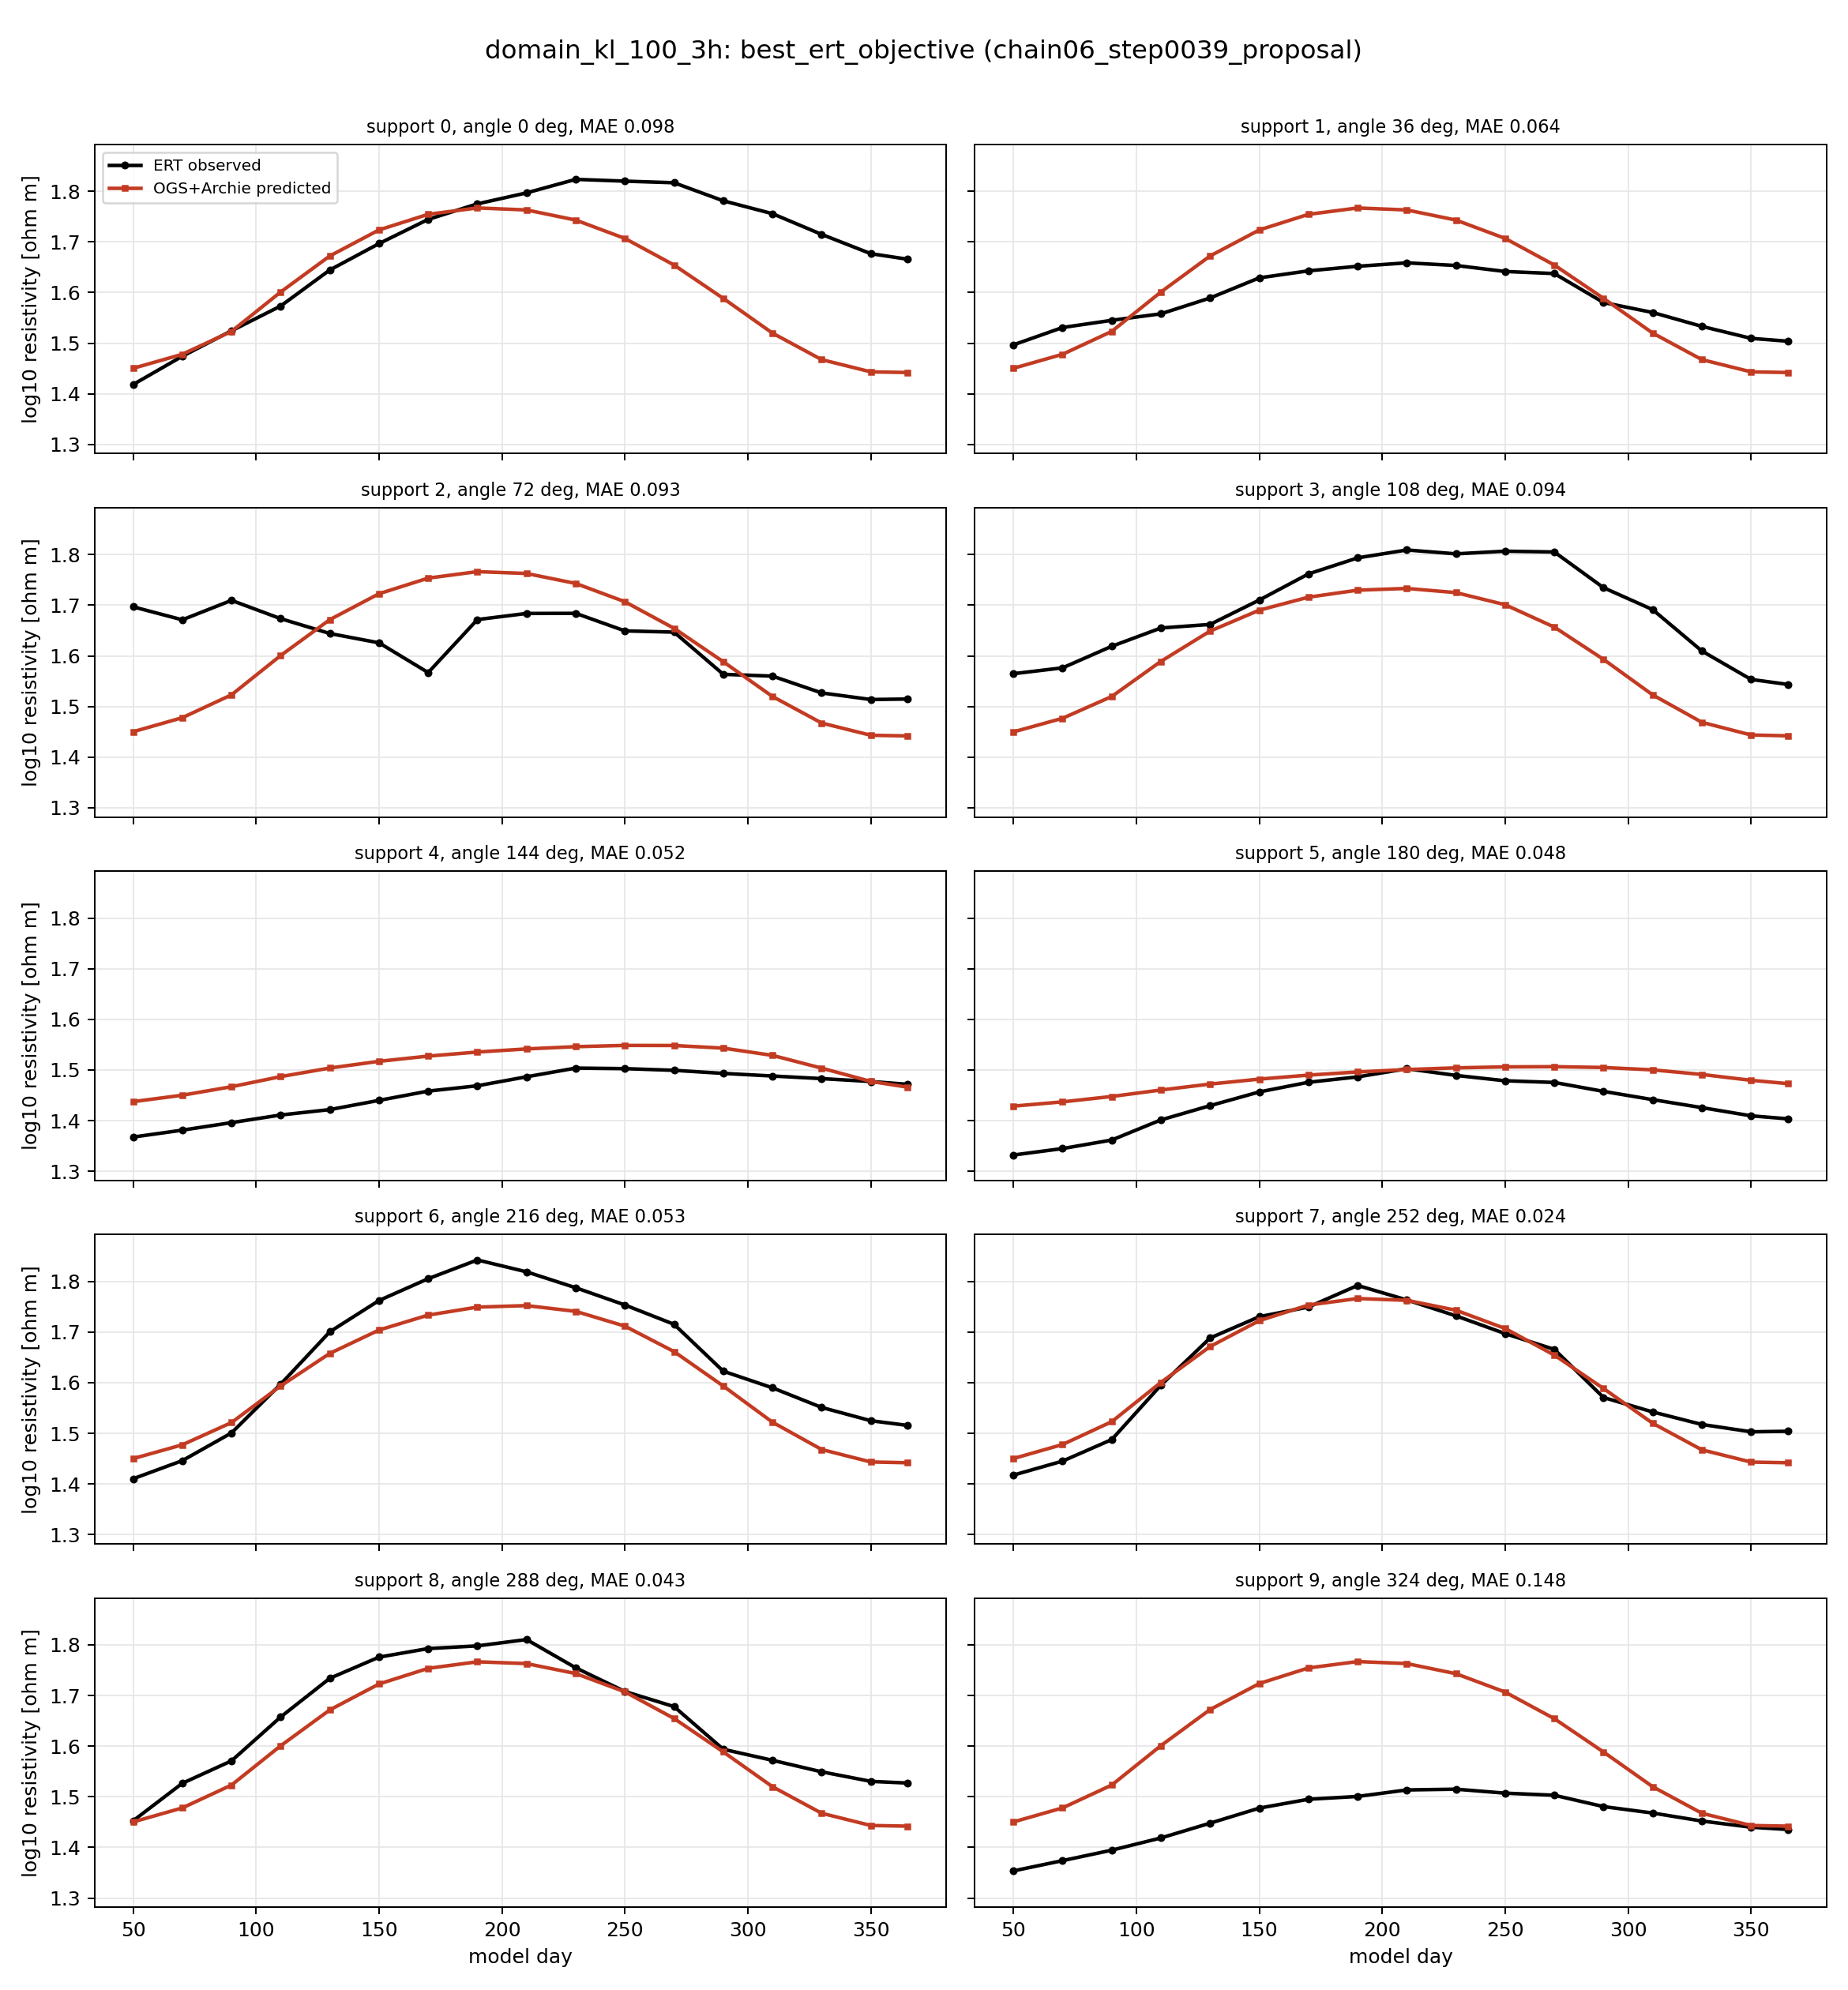
\includegraphics[width=0.98\linewidth]{domain_kl_100_3h_best_ert_objective_ert_support_fit.png}
\caption{First-year ERT evolution at the 10 support disks: observations against OGS+Archie predictions.}
\end{figure}

\section{Scalar Parameter Posteriors}

The posterior summary below uses the empirical MH state distribution in
\texttt{campaign\_samples.csv}, excluding the 16 \texttt{resume\_state} rows.
It excludes the 100 KL coefficients and cellwise permeability-field summaries,
but keeps the scalar parameters that control the tensor level/orientation,
Archie transform, porosity, NMR offset, ERT texture floor, and boundary curve.
Because this was a short 3-hour campaign, these are exploratory posterior
summaries rather than a convergence claim. The boundary suction scale and
offset were fixed in this campaign, so their posterior rows are degenerate.
The histogram panels are normalized as empirical posterior density estimates,
with KDE curves and prior PDFs overlaid for direct comparison. The two boundary
suction panels are zoomed fixed-value panels rather than sampled distributions.

\begin{table}[H]
\centering
\scriptsize
\resizebox{\linewidth}{!}{\begin{tabular}{lrrrrrr}
\toprule
Parameter & mean & std & p05 & median & p95 & best ERT \\
\midrule
k0 log10 k [m2] & -20.94 & 0.1908 & -21.23 & -20.97 & -20.67 & -21 \\
bedding angle [deg] & 141.6 & 1.027 & 140.1 & 141.5 & 143.7 & 140.7 \\
q = K22/K11 & 0.4234 & 0.03468 & 0.3612 & 0.4286 & 0.4751 & 0.4312 \\
homogeneous porosity & 0.1288 & 0.008242 & 0.1186 & 0.1259 & 0.1459 & 0.1446 \\
Archie log10 a & 0.7307 & 0.0951 & 0.57 & 0.7549 & 0.8778 & 0.7858 \\
Archie exponent b & -0.7428 & 0.08711 & -0.8868 & -0.7337 & -0.6078 & -0.7388 \\
NMR bound water & 0.04788 & 0.006391 & 0.03494 & 0.04873 & 0.05783 & 0.05352 \\
ERT texture floor log10 & 0.1603 & 0.05592 & 0.08355 & 0.153 & 0.2719 & 0.2837 \\
boundary shift [d] & 105.1 & 17.11 & 77.96 & 105.4 & 132.6 & 89.04 \\
boundary suction scale & 1 & 0 & 1 & 1 & 1 & 1 \\
boundary suction offset [MPa] & 0 & 0 & 0 & 0 & 0 & 0 \\
\bottomrule
\end{tabular}
}
\caption{Scalar parameter posterior summaries from 1205 non-resume MH states. The best-ERT column marks \texttt{chain06\_step0039\_proposal}.}
\end{table}

\begin{figure}[H]
\centering
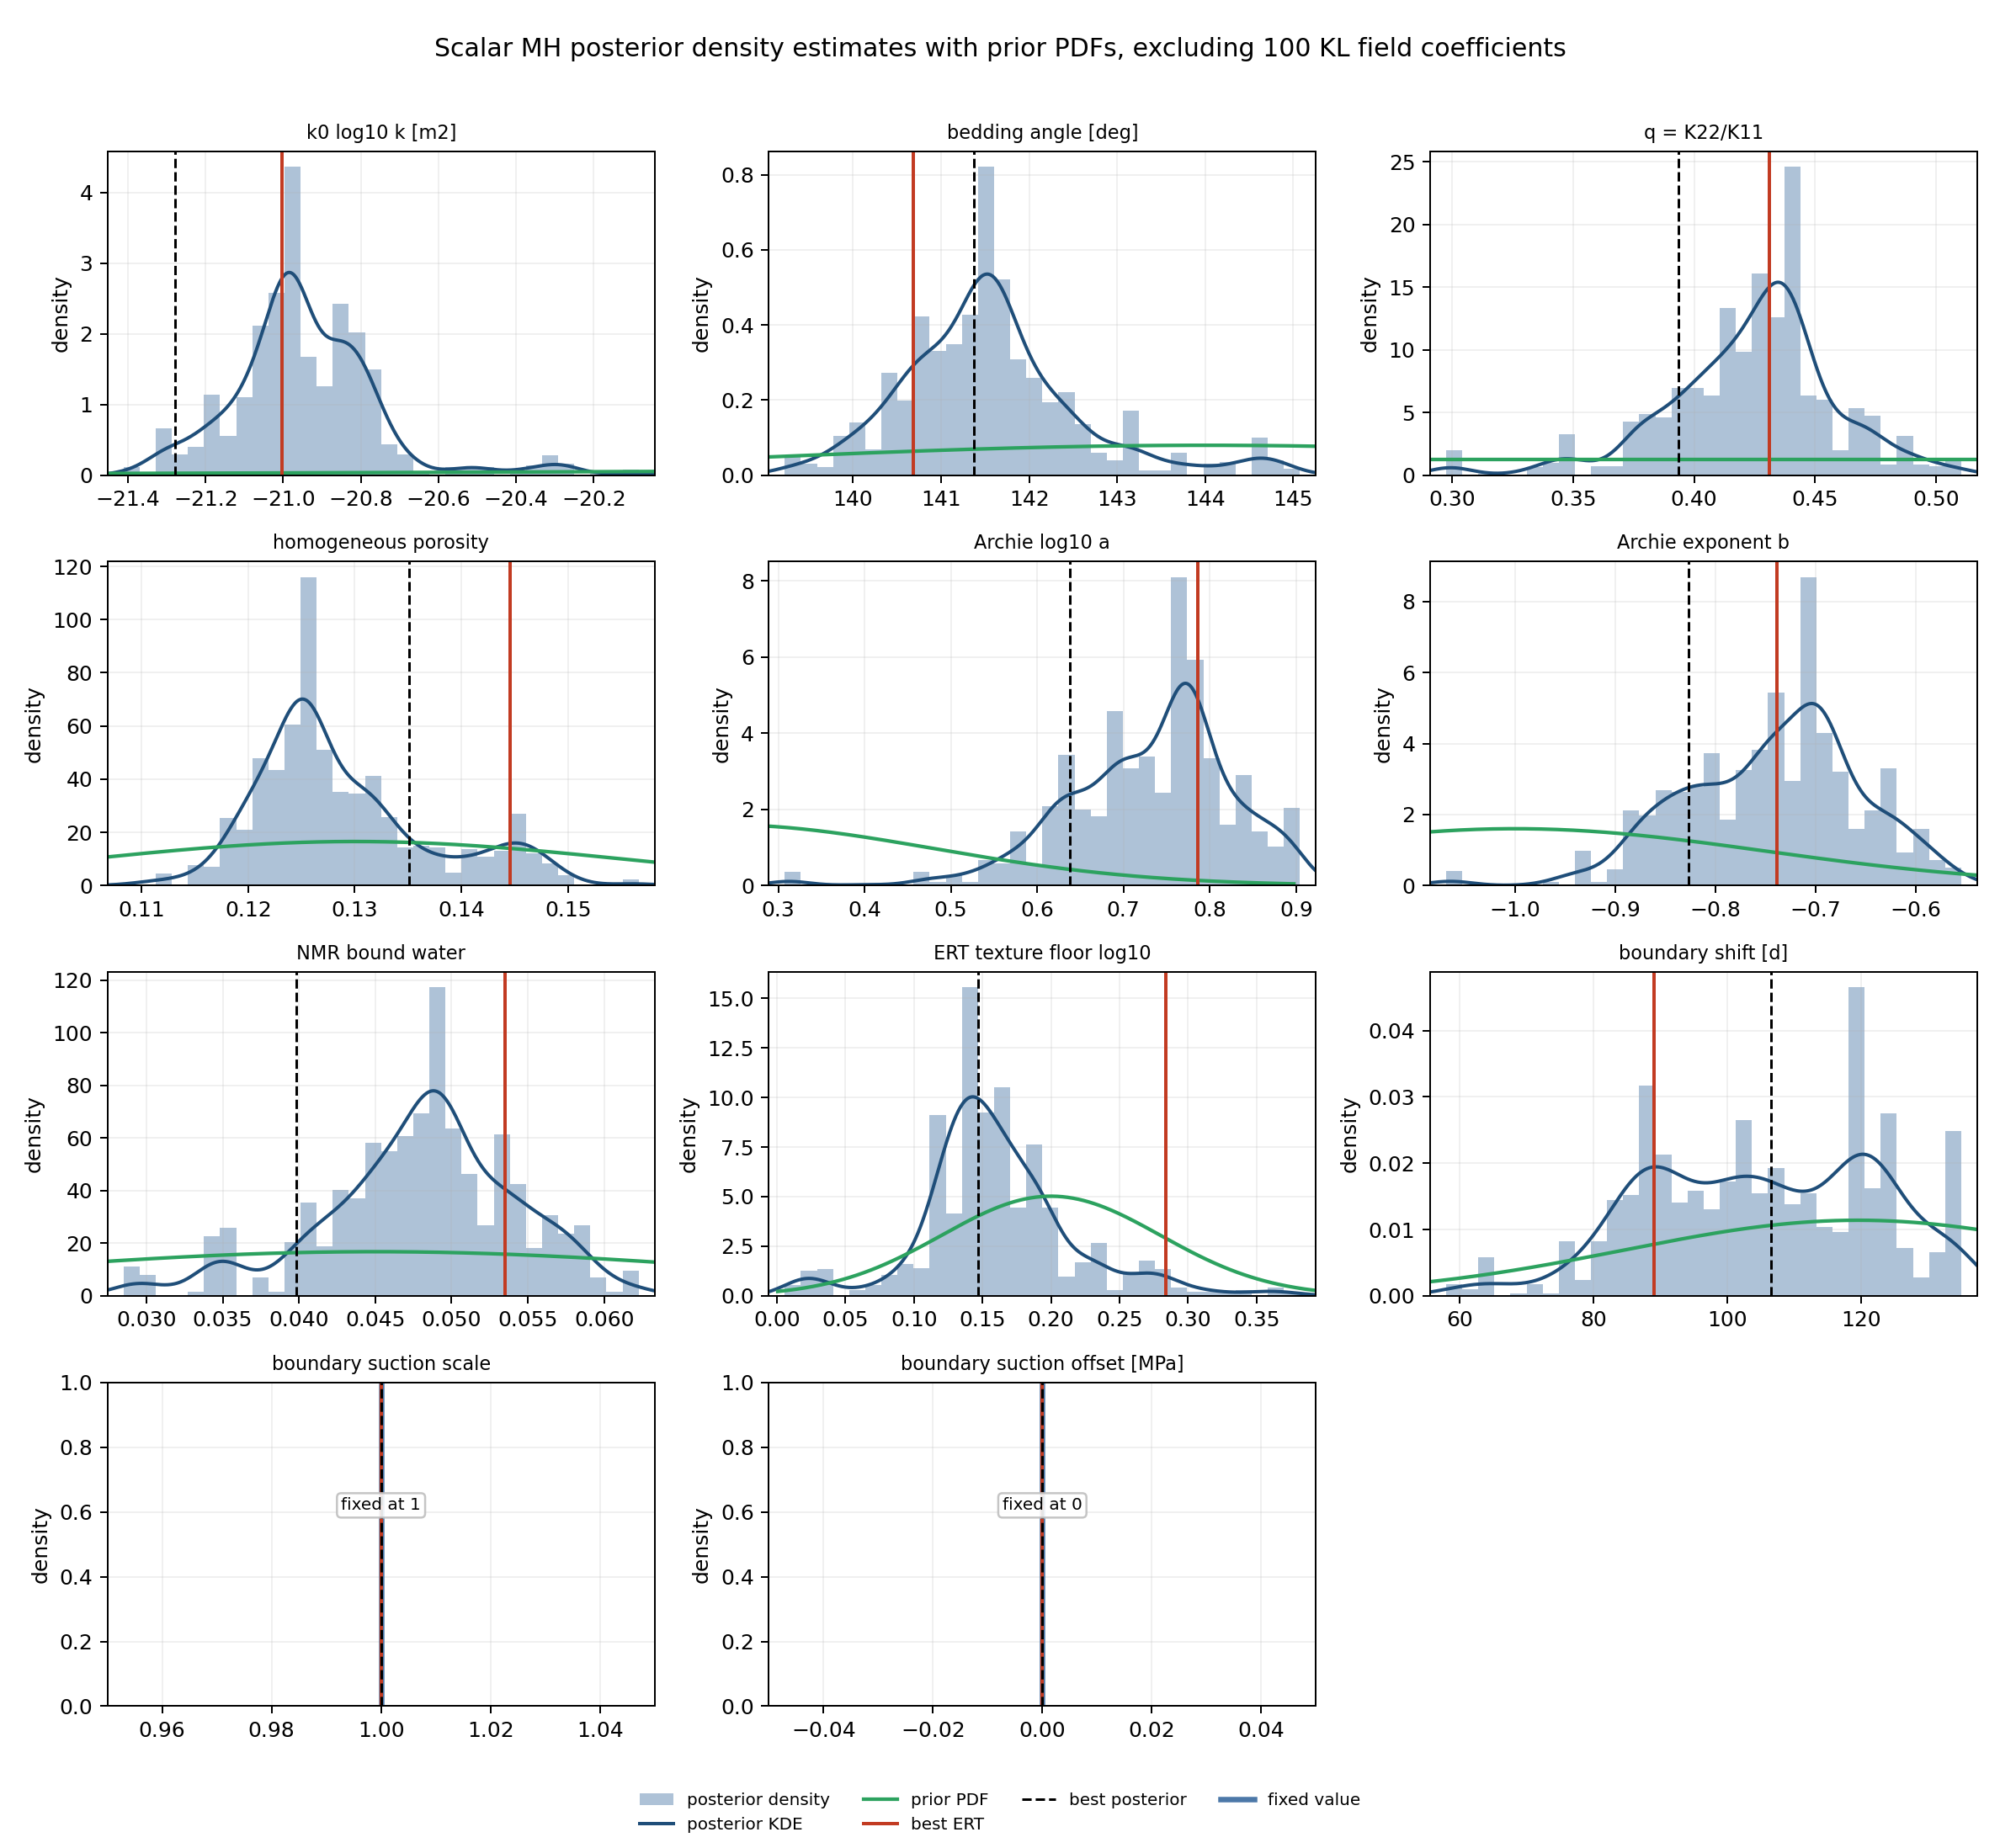
\includegraphics[width=0.98\linewidth]{domain_kl_100_3h_scalar_parameter_posterior_histograms.png}
\caption{Empirical posterior density estimates for scalar parameters. Blue bars are normalized posterior densities, dark-blue curves are KDE estimates, green curves are prior PDFs, red lines mark the best ERT candidate, and dashed black lines mark the best posterior candidate. Fixed boundary suction scale and offset are shown as zoomed fixed-value panels.}
\end{figure}

\begin{figure}[H]
\centering
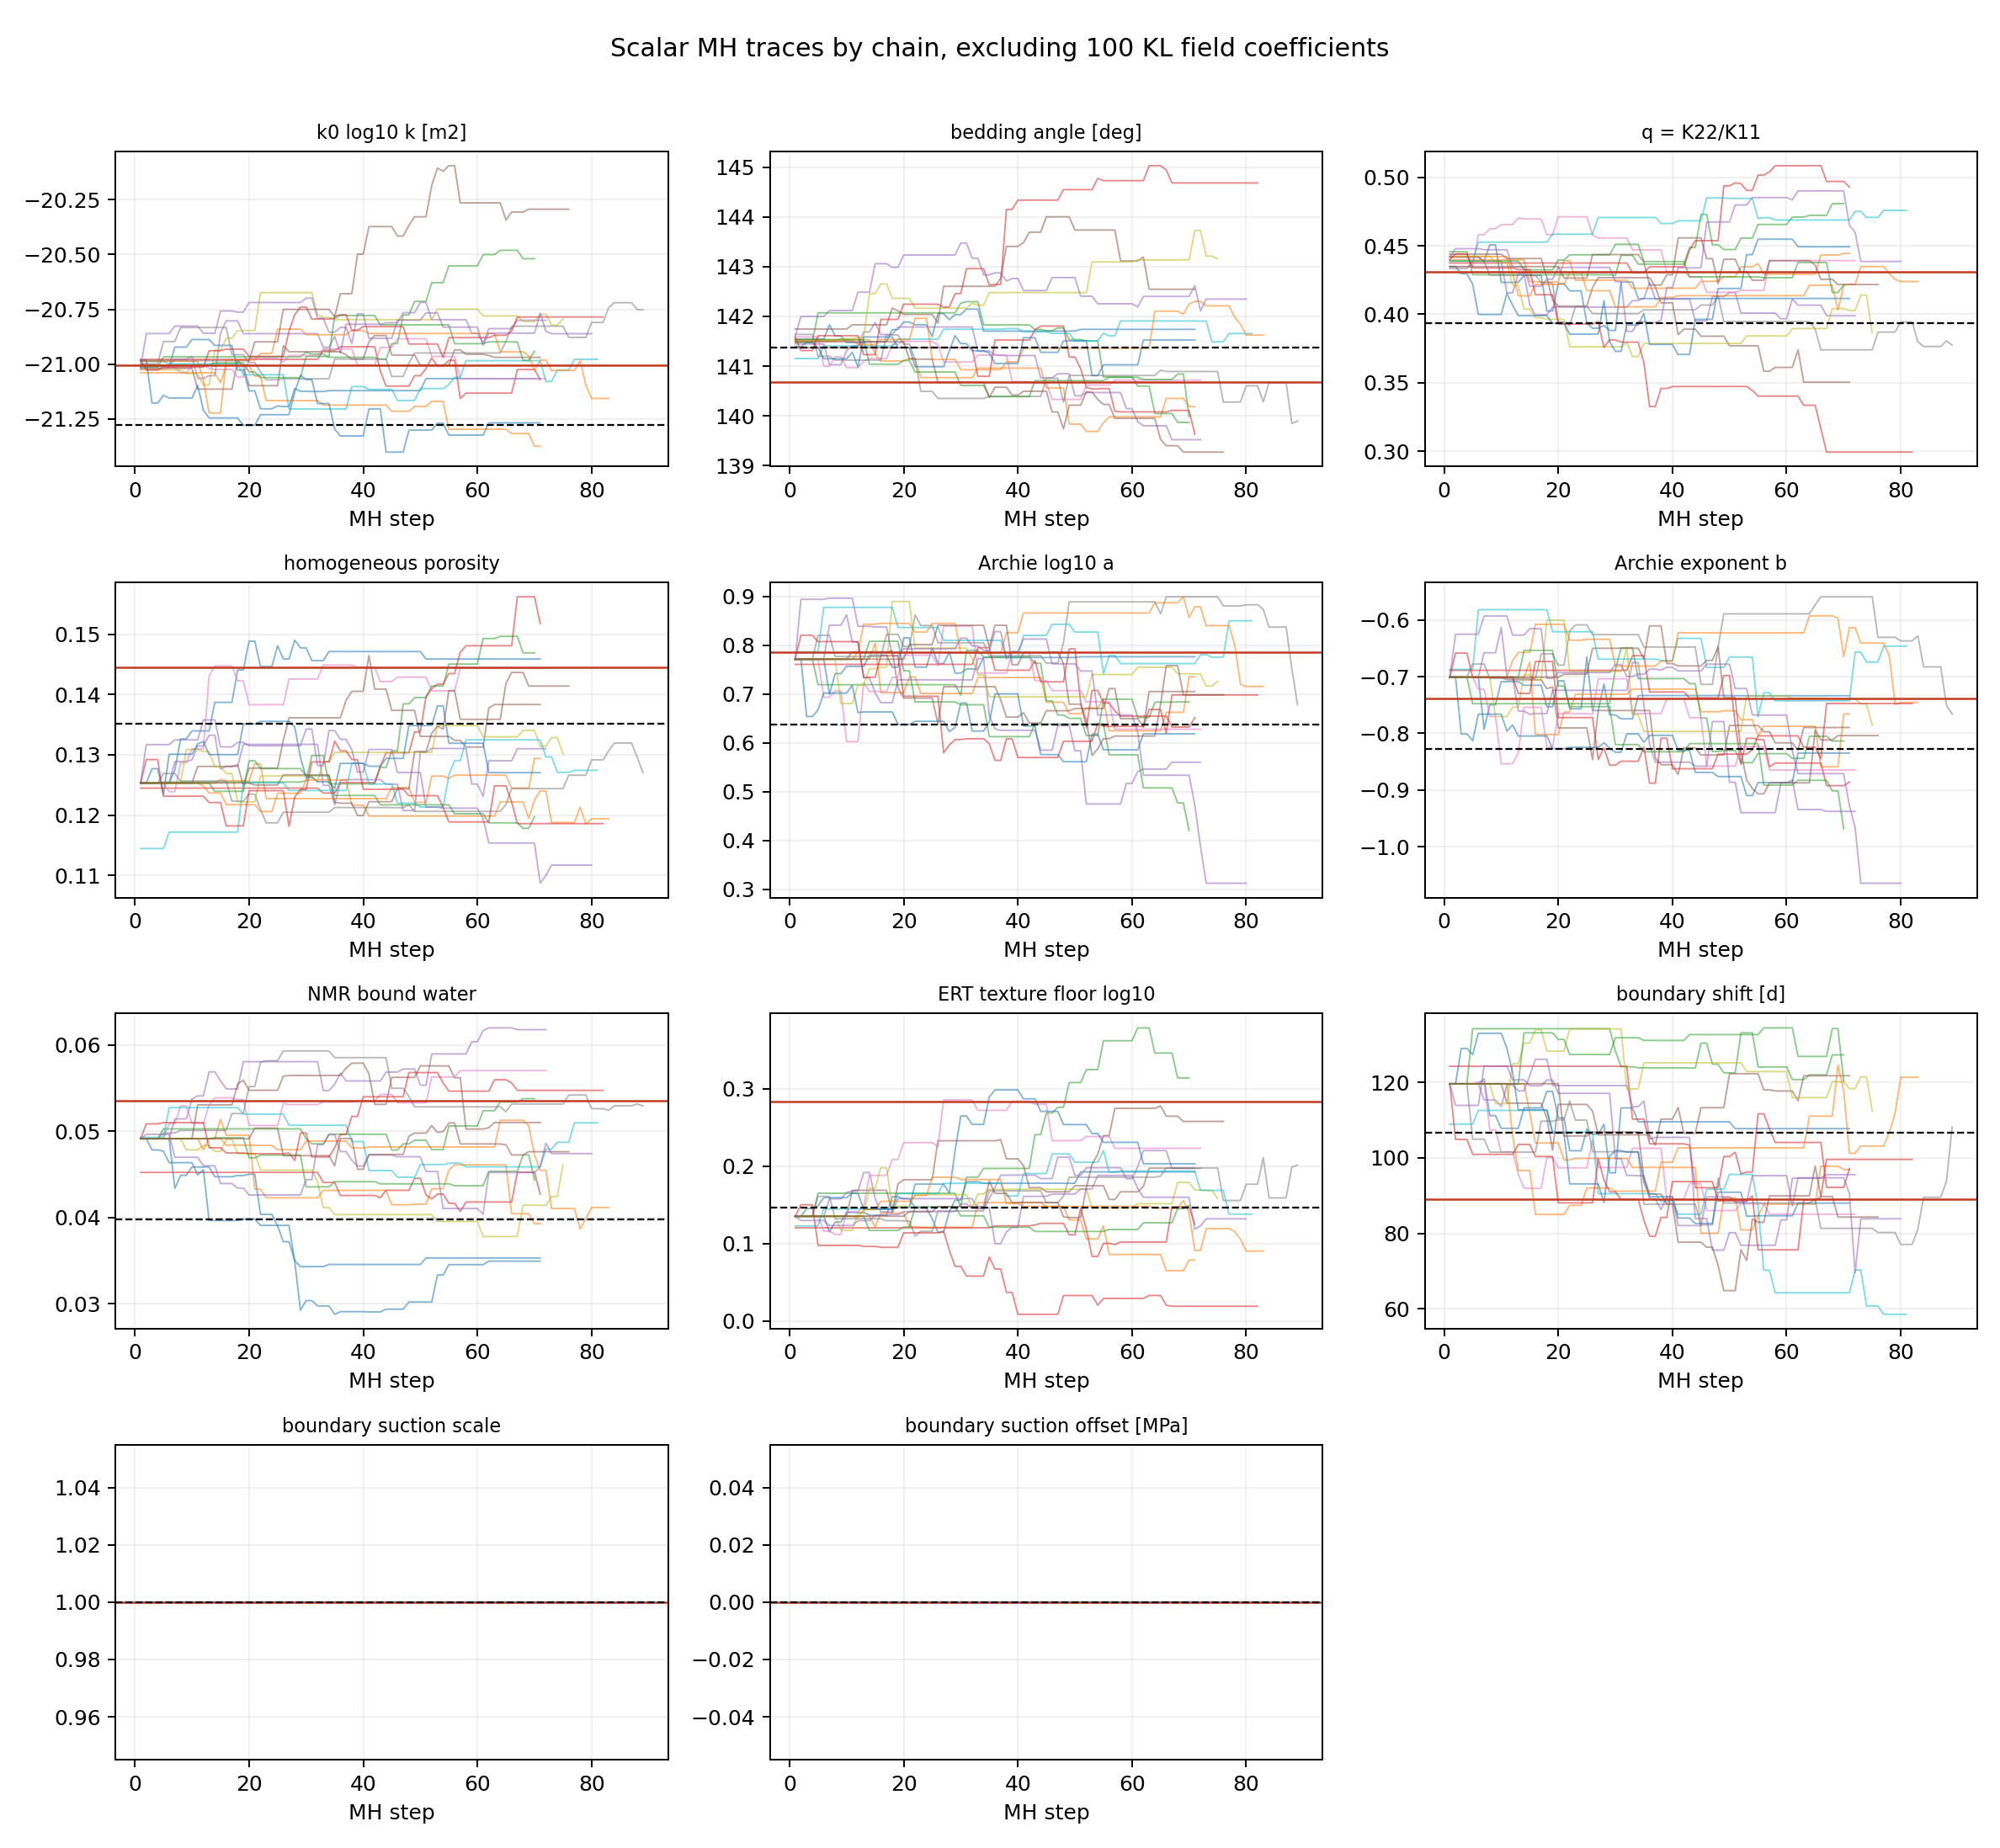
\includegraphics[width=0.98\linewidth]{domain_kl_100_3h_scalar_parameter_posterior_traces.png}
\caption{Scalar parameter MH traces by chain. Red horizontal lines mark the best ERT value; dashed black lines mark the best posterior value.}
\end{figure}

\section{Permeability Field}

\begin{figure}[H]
\centering
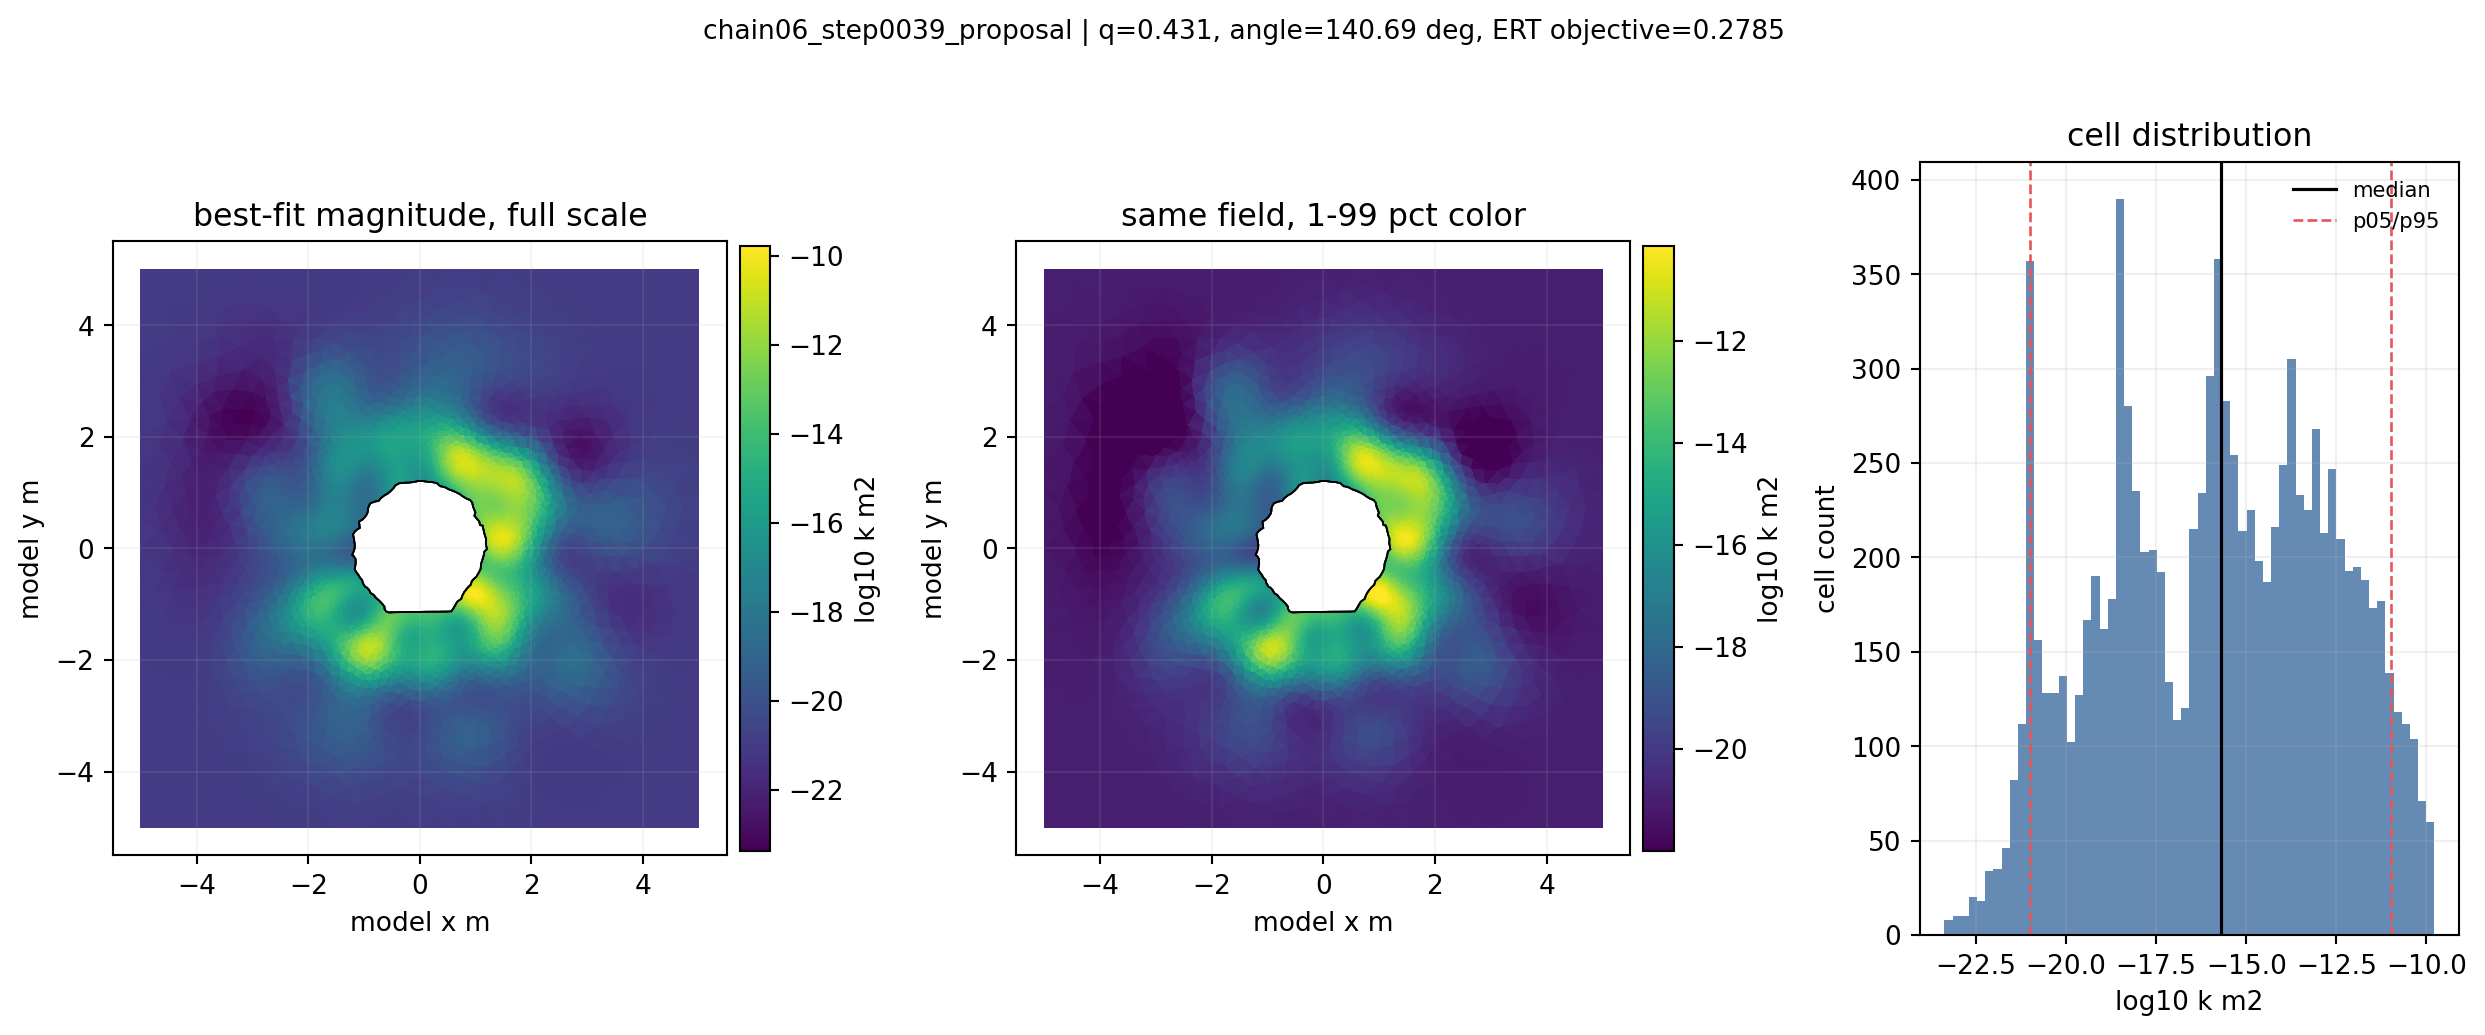
\includegraphics[width=0.98\linewidth]{domain_kl_100_3h_best_ert_objective_permeability_magnitude.png}
\caption{Best-fit scalar intrinsic-permeability magnitude recovered from tensor \texttt{k\_i\_rd} as \(\mathrm{trace}(K_i)/(1+q)\).}
\end{figure}

\begin{table}[H]
\centering
\begin{tabular}{ll}
\toprule
Field statistic & log10 m2 \\
\midrule
Minimum & -23.376174 \\
p05 & -21.011958 \\
Median & -15.712623 \\
Mean & -15.851041 \\
p95 & -10.987349 \\
Maximum & -9.779248 \\
\bottomrule
\end{tabular}
\caption{Best-fit scalar permeability magnitude distribution on mesh cells.}
\end{table}

\section{Circular ERT Error Diagnostics}

\begin{figure}[H]
\centering
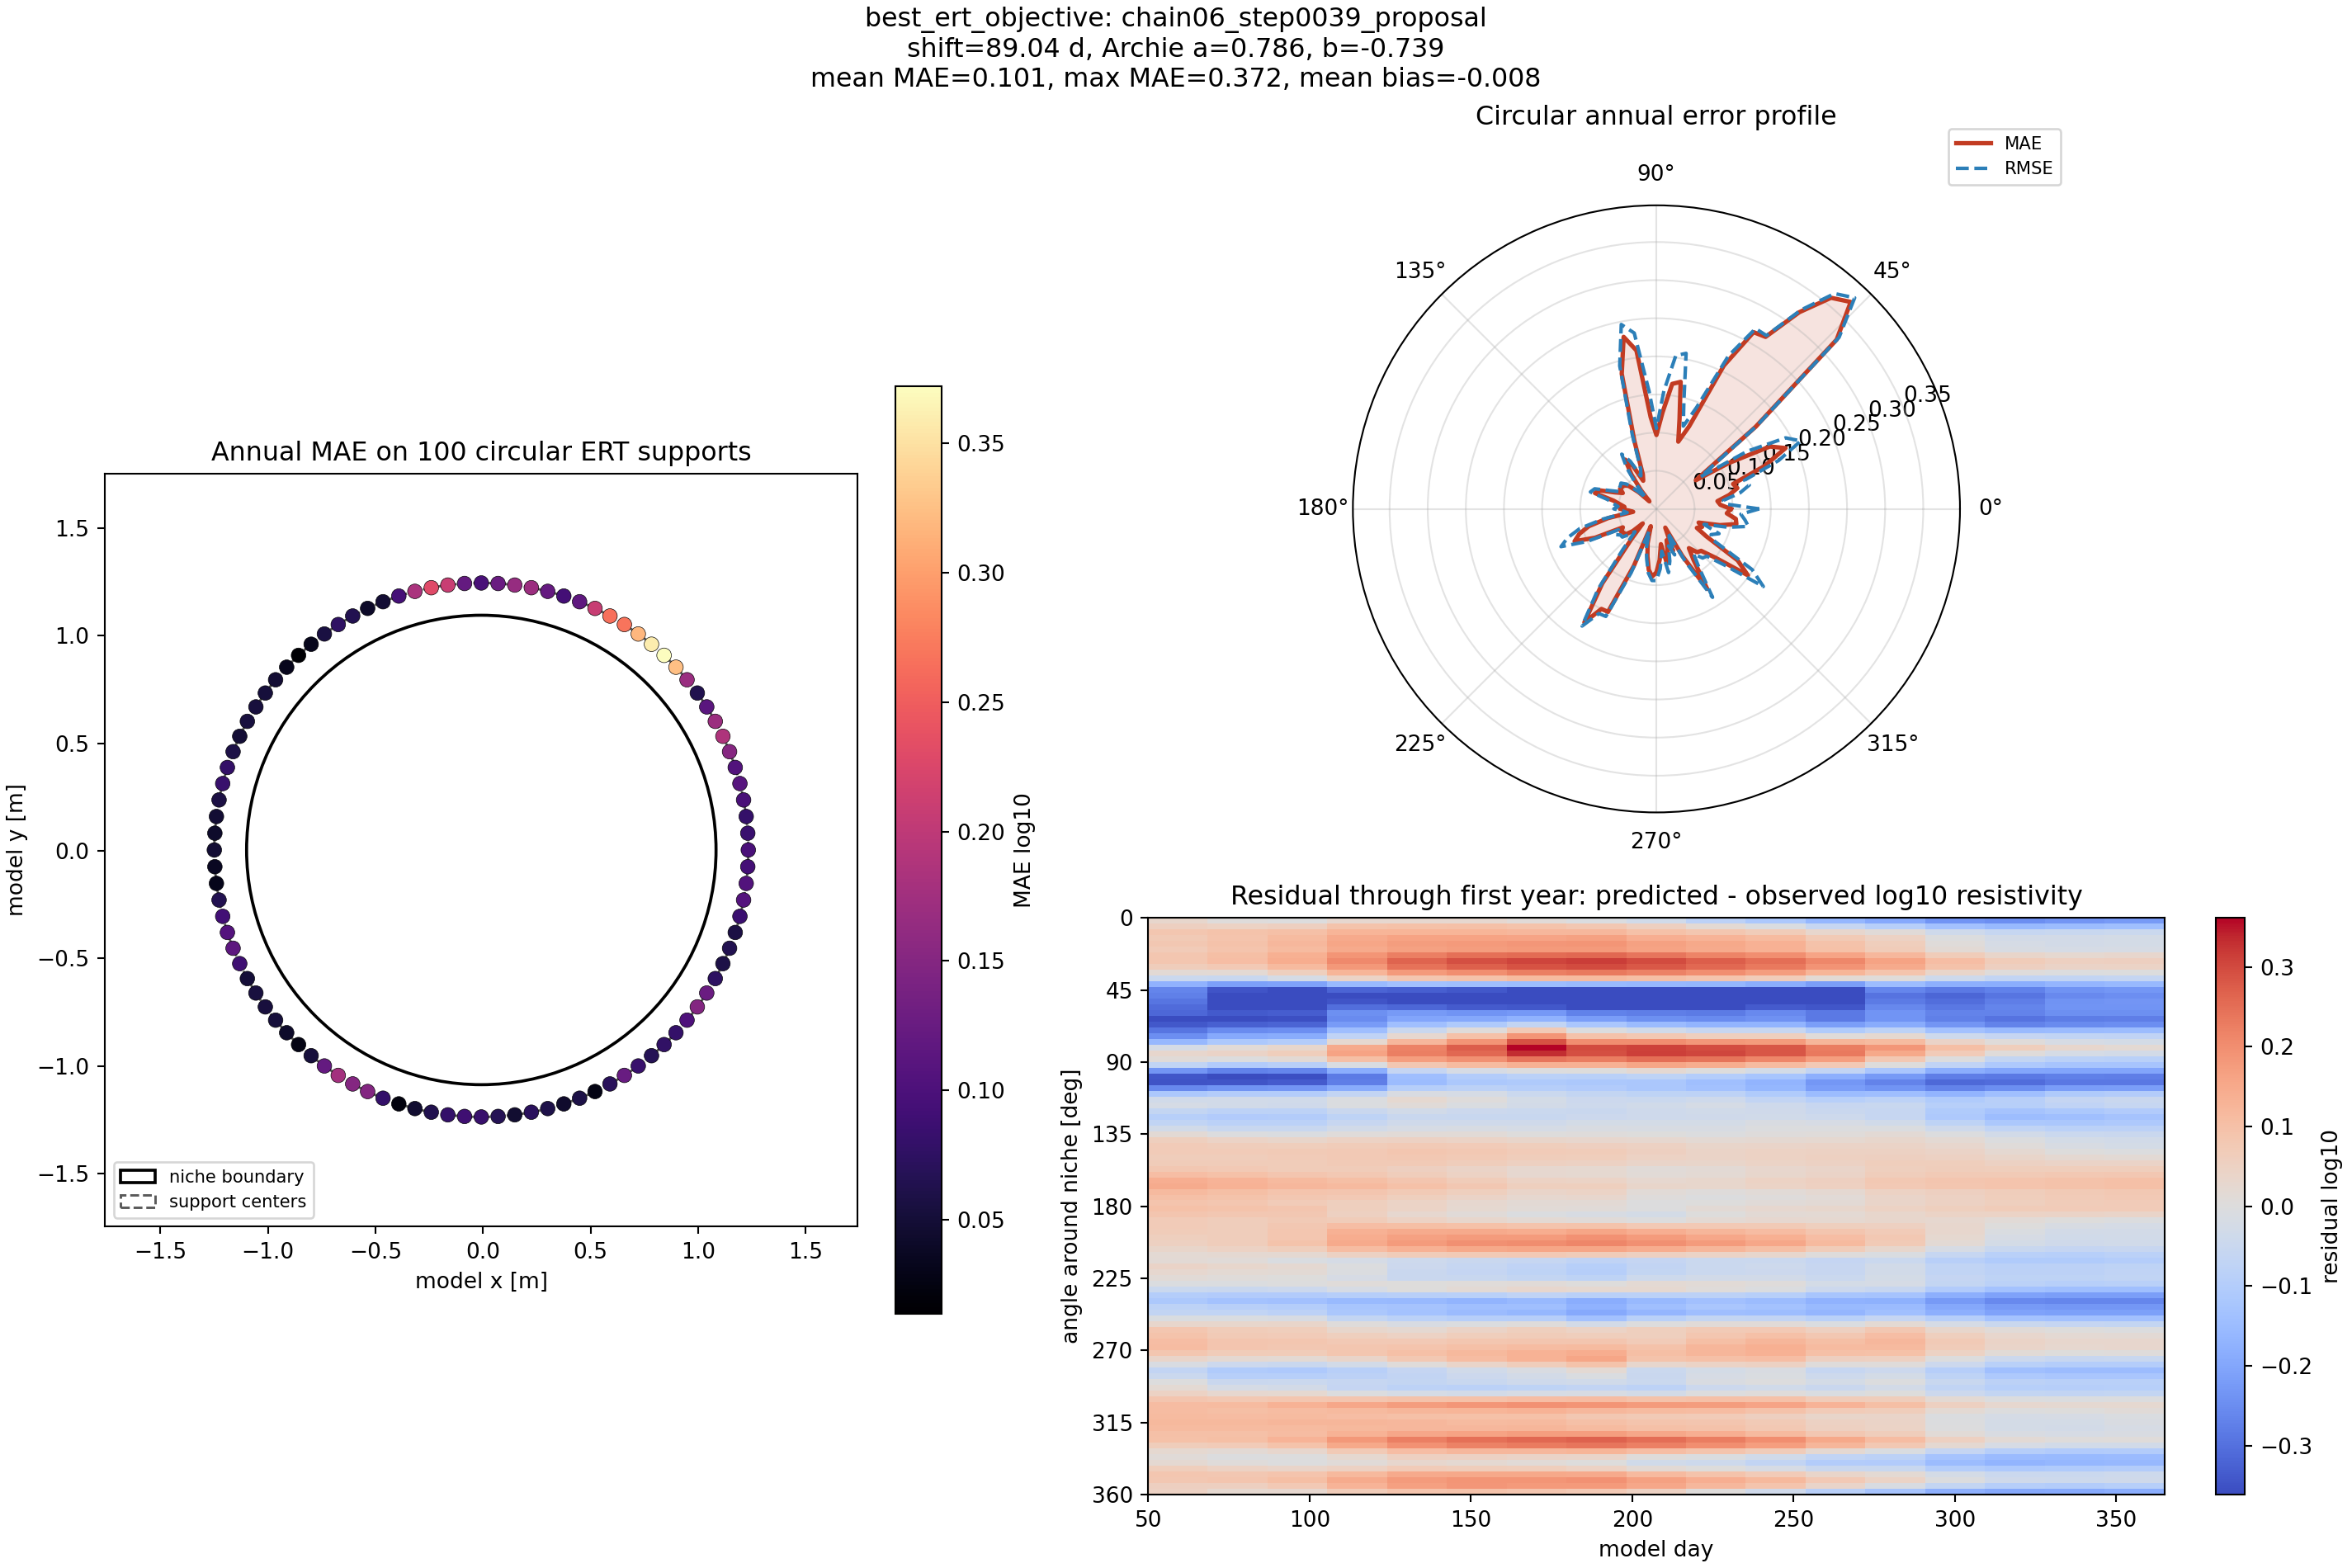
\includegraphics[width=0.98\linewidth]{domain_kl_100_3h_ert100_circle_error_profile_best_ert_objective.png}
\caption{Annual error profile on 100 circular ERT support disks around the niche at approximately 15 cm depth.}
\end{figure}

\begin{figure}[H]
\centering
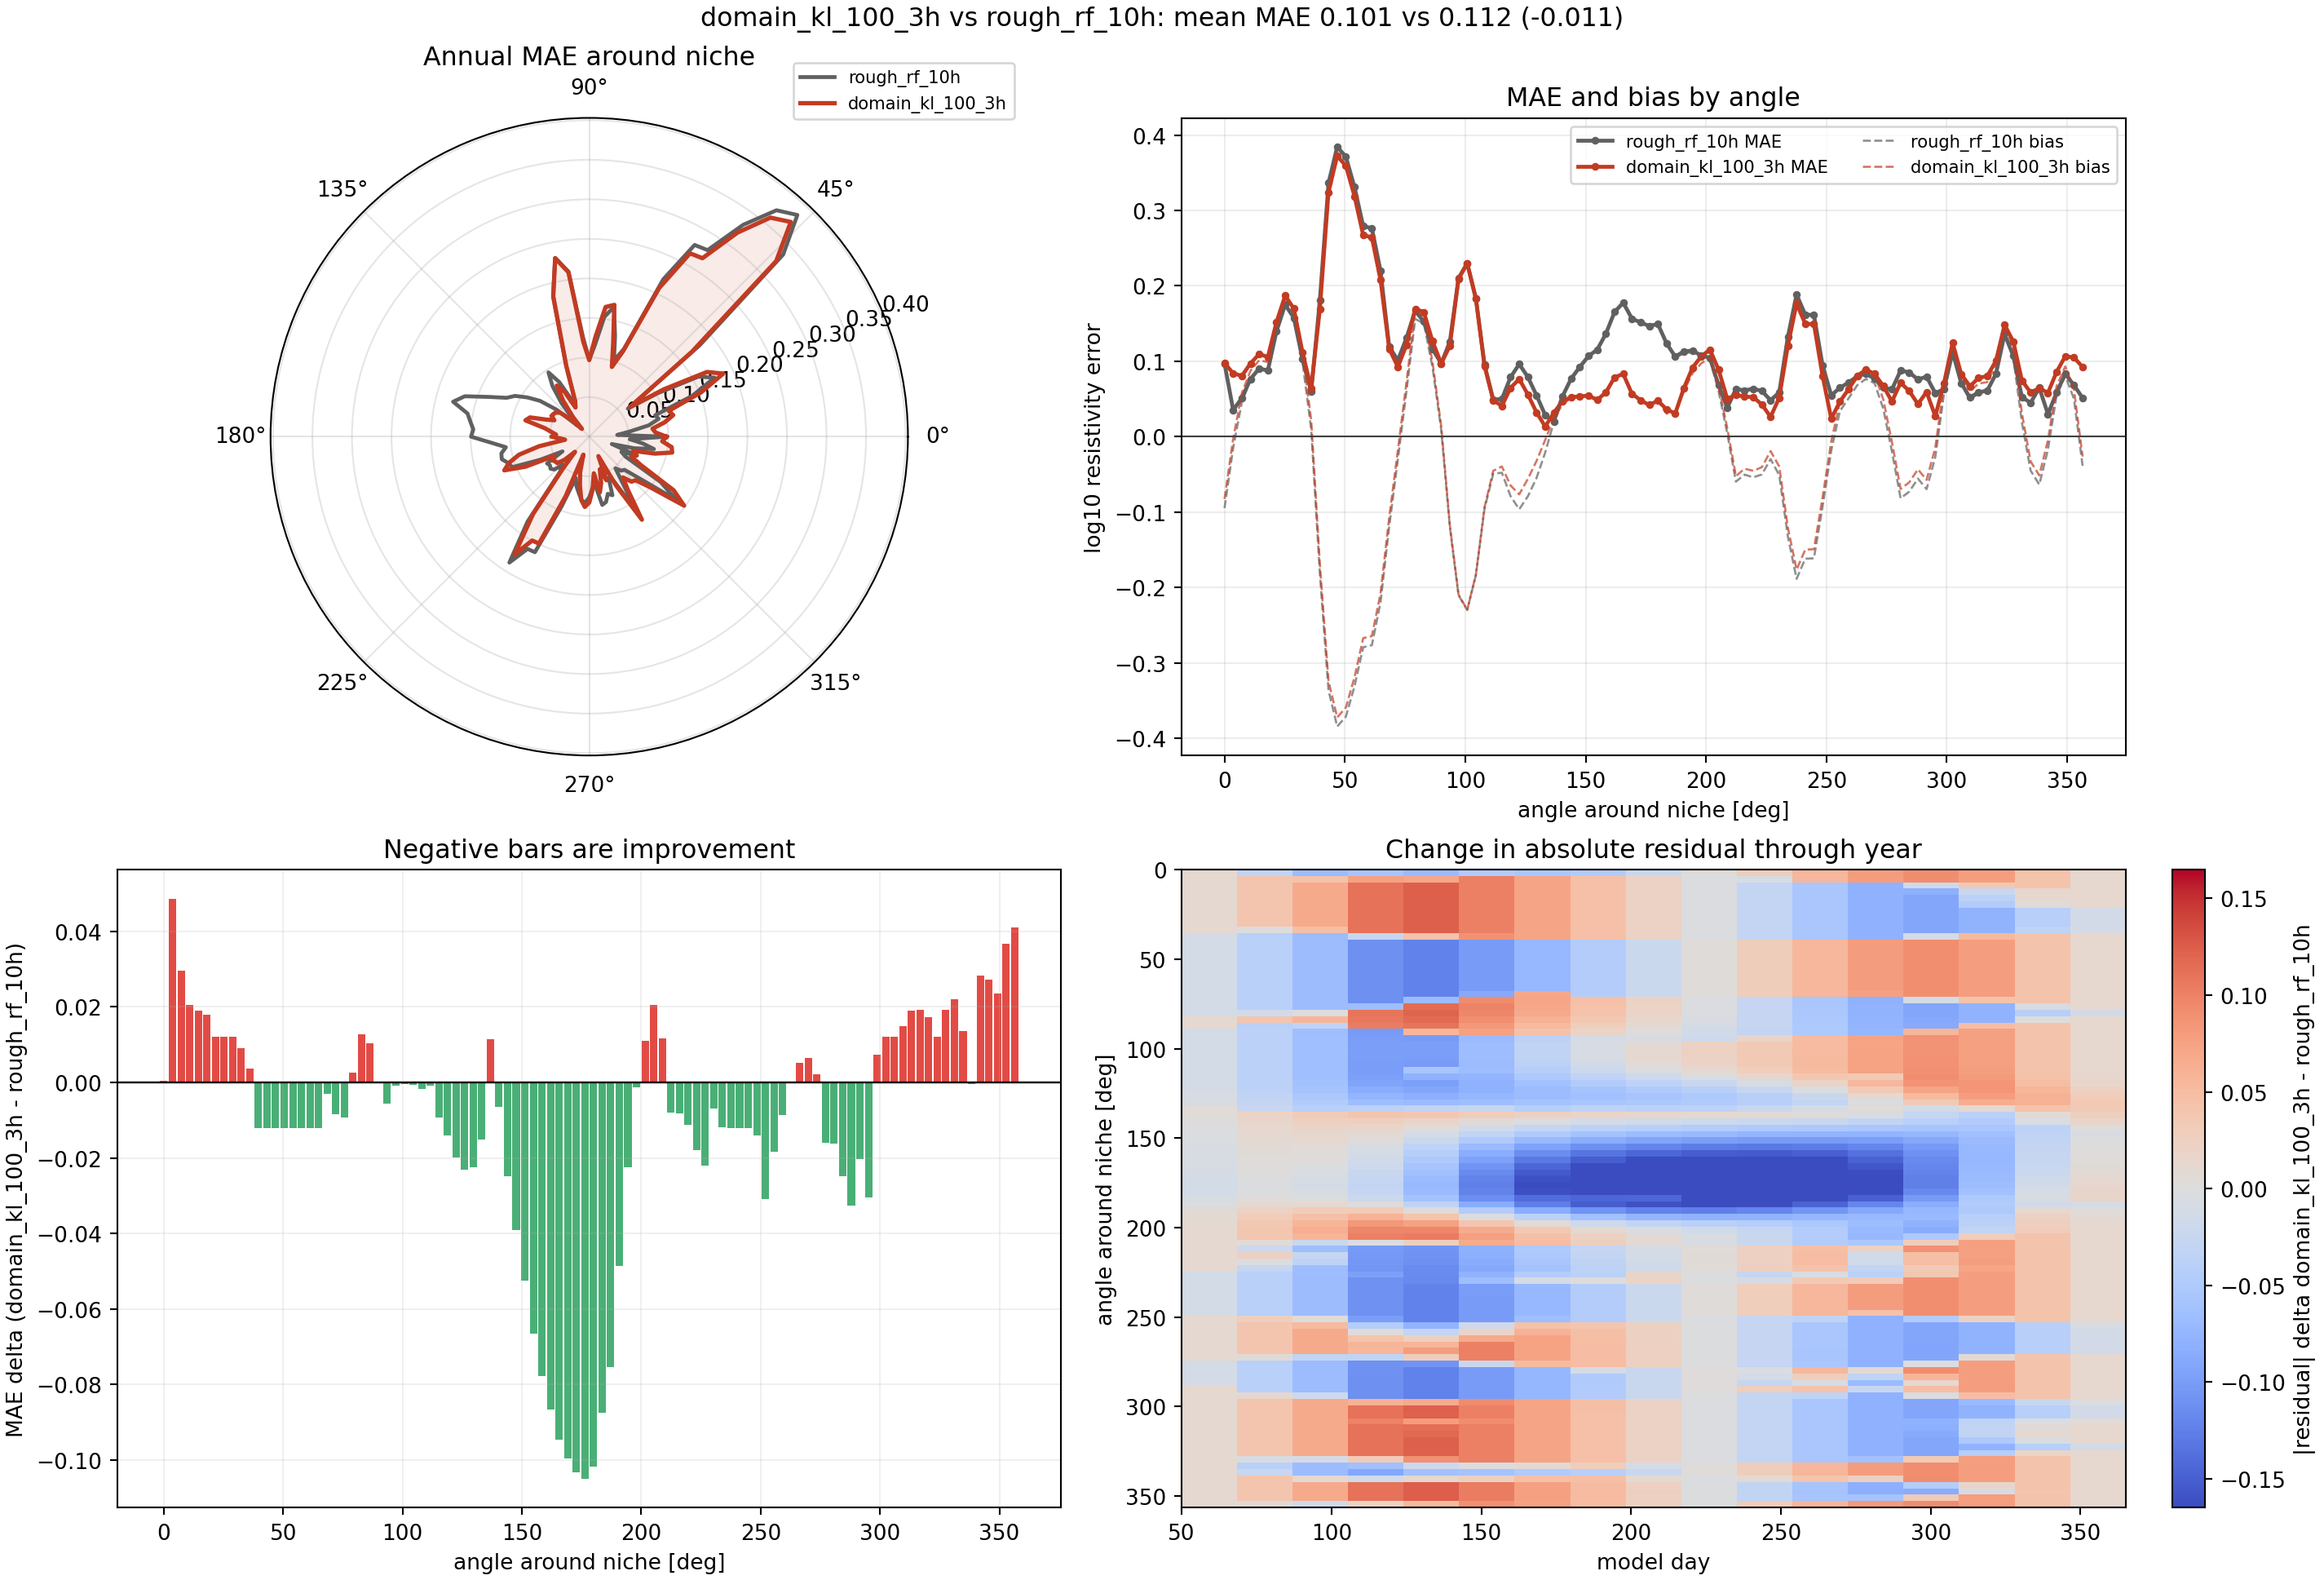
\includegraphics[width=0.98\linewidth]{domain_kl_100_3h_vs_rough_rf_10h_ert100_radial_error_comparison.png}
\caption{Comparison against the previous rough-RF 10-hour baseline. Negative bars indicate lower MAE for the new domain-KL campaign.}
\end{figure}

\begin{table}[H]
\centering
\begin{tabular}{lll}
\toprule
Metric & Rough-RF 10h & Domain-KL 100 3h \\
\midrule
Mean radial MAE & 0.111878 & 0.101334 \\
Maximum radial MAE & 0.384404 & 0.372321 \\
Mean MAE change & \multicolumn{2}{c}{-0.010545} \\
Improved supports & \multicolumn{2}{c}{62 / 100} \\
Worst remaining direction & \multicolumn{2}{c}{near 45 deg} \\
Largest improvement direction & \multicolumn{2}{c}{176.4 deg} \\
\bottomrule
\end{tabular}
\caption{100-point circular ERT diagnostic summary.}
\end{table}

\section{Commands And Artifacts}

The final report bundle was generated with:
\begin{verbatim}
python3 scripts/write_domain_kl_campaign_report.py \
  --campaign-id ert10_support_365d_domain_kl_100_3h_native_s1_v1 \
  --label domain_kl_100_3h

python3 scripts/plot_domain_kl_scalar_posteriors.py \
  --campaign-id ert10_support_365d_domain_kl_100_3h_native_s1_v1 \
  --label domain_kl_100_3h
\end{verbatim}

This PDF was compiled with:
\begin{verbatim}
cd report
pdflatex -interaction=nonstopmode -halt-on-error \
  domain_kl_100_3h_final_report.tex
\end{verbatim}

Primary report tables are in \texttt{tables/}; final plots are in
\texttt{figures/}. Raw campaign tables and the Markdown companion remain in
the original untracked run outputs.

\end{document}
